\subsubsection*{Visitor Pattern}\label{subs:visit}
The visitor pattern is not only used to traverse the parse tree provided by ANTLR, but also the \acrshort{ast} created in the compiler.
The visitor pattern is implemented throughout the compiler, to create the \acrshort{ast} from the parse tree and for traversing the \acrshort{ast}.
As such the visitor pattern defines the structure of the compiler, and thus understanding the benefit from using the pattern is important.
The visitor pattern is described by the Gang of Four, authors of ``Design Patterns: Elements of Reusable Object-Oriented Software'' as:
``a design pattern that separates a set of structured data from the functionality that may be performed upon it.''. \citep{GOF}

In the tree walk for the parse tree, the visitor should convert the parse tree into a \acrshort{ast}.
This entails that each different node in the parse tree must be visited to find the information needed to create the \acrshort{ast}.

Through use of the visitor pattern the functionality is separated from the classes they are performed upon. 
Instead the functionality is on a visitor class implementing the visitor interface, which means different visitors can be made, which all do different computations while traversing the tree.\todo{måske tasks i stedet for computations. MP}
Each class in the tree have an \texttt{accept()} method that allows them to call the visitor in question with itself as an argument.
This allows the ability of adding new operations without changing the original data structure, and also without changing other visitors.
This also serves well when using a iterative development method.
Another benefit is that a single visitor object is used to visit all the classes in the tree.
This visitor can therefore maintain a state between calls to individual data objects, which can be used to save information in an outer scope from the different visit calls.
\myref{image:visitor} shows an UML diagram of the visitor pattern.
This diagram is from a C\# representation, and while the idea is the same the exact implementation is not identical to the one used in the compiler for \gls{gamble}.
Take note of the classes ``ConcreteElement'' and ``ConcreteVisitor''.
The ``ConcreteElement'' represents the different kinds of nodes in a given tree.
The ``ConcreteVisitor'' represents the different kind of visitors implemented.
A visitor will make sure that the children of the node is traversed in the correct way, and will at the same time also do other computations, e.g. pretty printing or checking the source code for errors.\todo{Skal vi komme med andre eksempler her ? Såsom, type checking or code generating?}
A visitor must implement a method to visit every single ``ConcreteElement'' which exist in the tree.
As can be seen on \myref{image:visitor} ``ConcreteVisitorA'' and ``ConcreteVisitorB'', both implement a visit method for the ``ConcreteElements'' A and B.
In the next section, the implementation of creating the \acrshort{ast} from the parse tree using the visitor pattern will be presented.

\begin{figure}[!ht]
\centering
 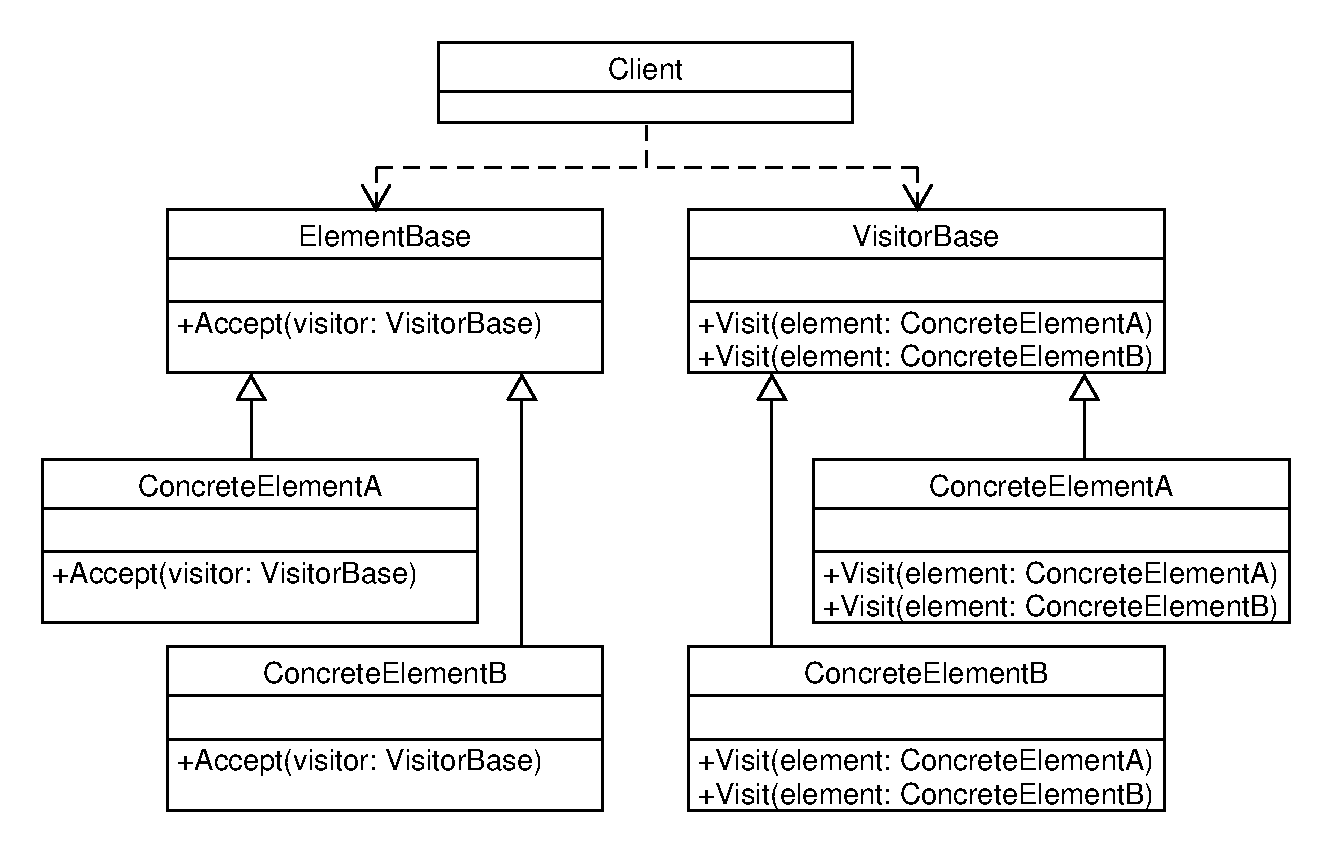
\includegraphics[width=1\textwidth]{figures/ClassDiagrams/VisitorPattern.pdf} % trim=4.85cm 15cm 0.85cm 1cm
\caption{An UML diagram for the implementation of the visitor pattern.}\label{image:visitor}
\vspace{-15pt}
\end{figure}
\todo[inline]{har vi selv lavet figuren? MP - Ja den har jeg lavet :) men der skal nok en kilde på så man kan se hvor vi har det fra, Marc found it. - Søren}

\subsection{Creating the \acrshort{ast}}\label{CreatingAst}

The goal for the \acrshort{ast} is to decrease the information in the tree.
The hidden information is then contained in fields created for the respective classes.
Rather than having the information as fields one could also choose to have this information as children of the nodes.
This would mean that to find the information one would have to run through the children of the node whereas the method chosen for this compiler, this information is kept on the fields of a node.
The advantage being that the information is kept together without clustering the tree.
All the nodes of the \acrshort{ast} have been designed with this in mind.
For example on figure \myref{image:ASTDecl} a class structure can be seen, which consists of all the classes needed to express a declaration on the tree.
A declaration could be \texttt{int a = 5;}.

\begin{figure}[!ht]
\centering
 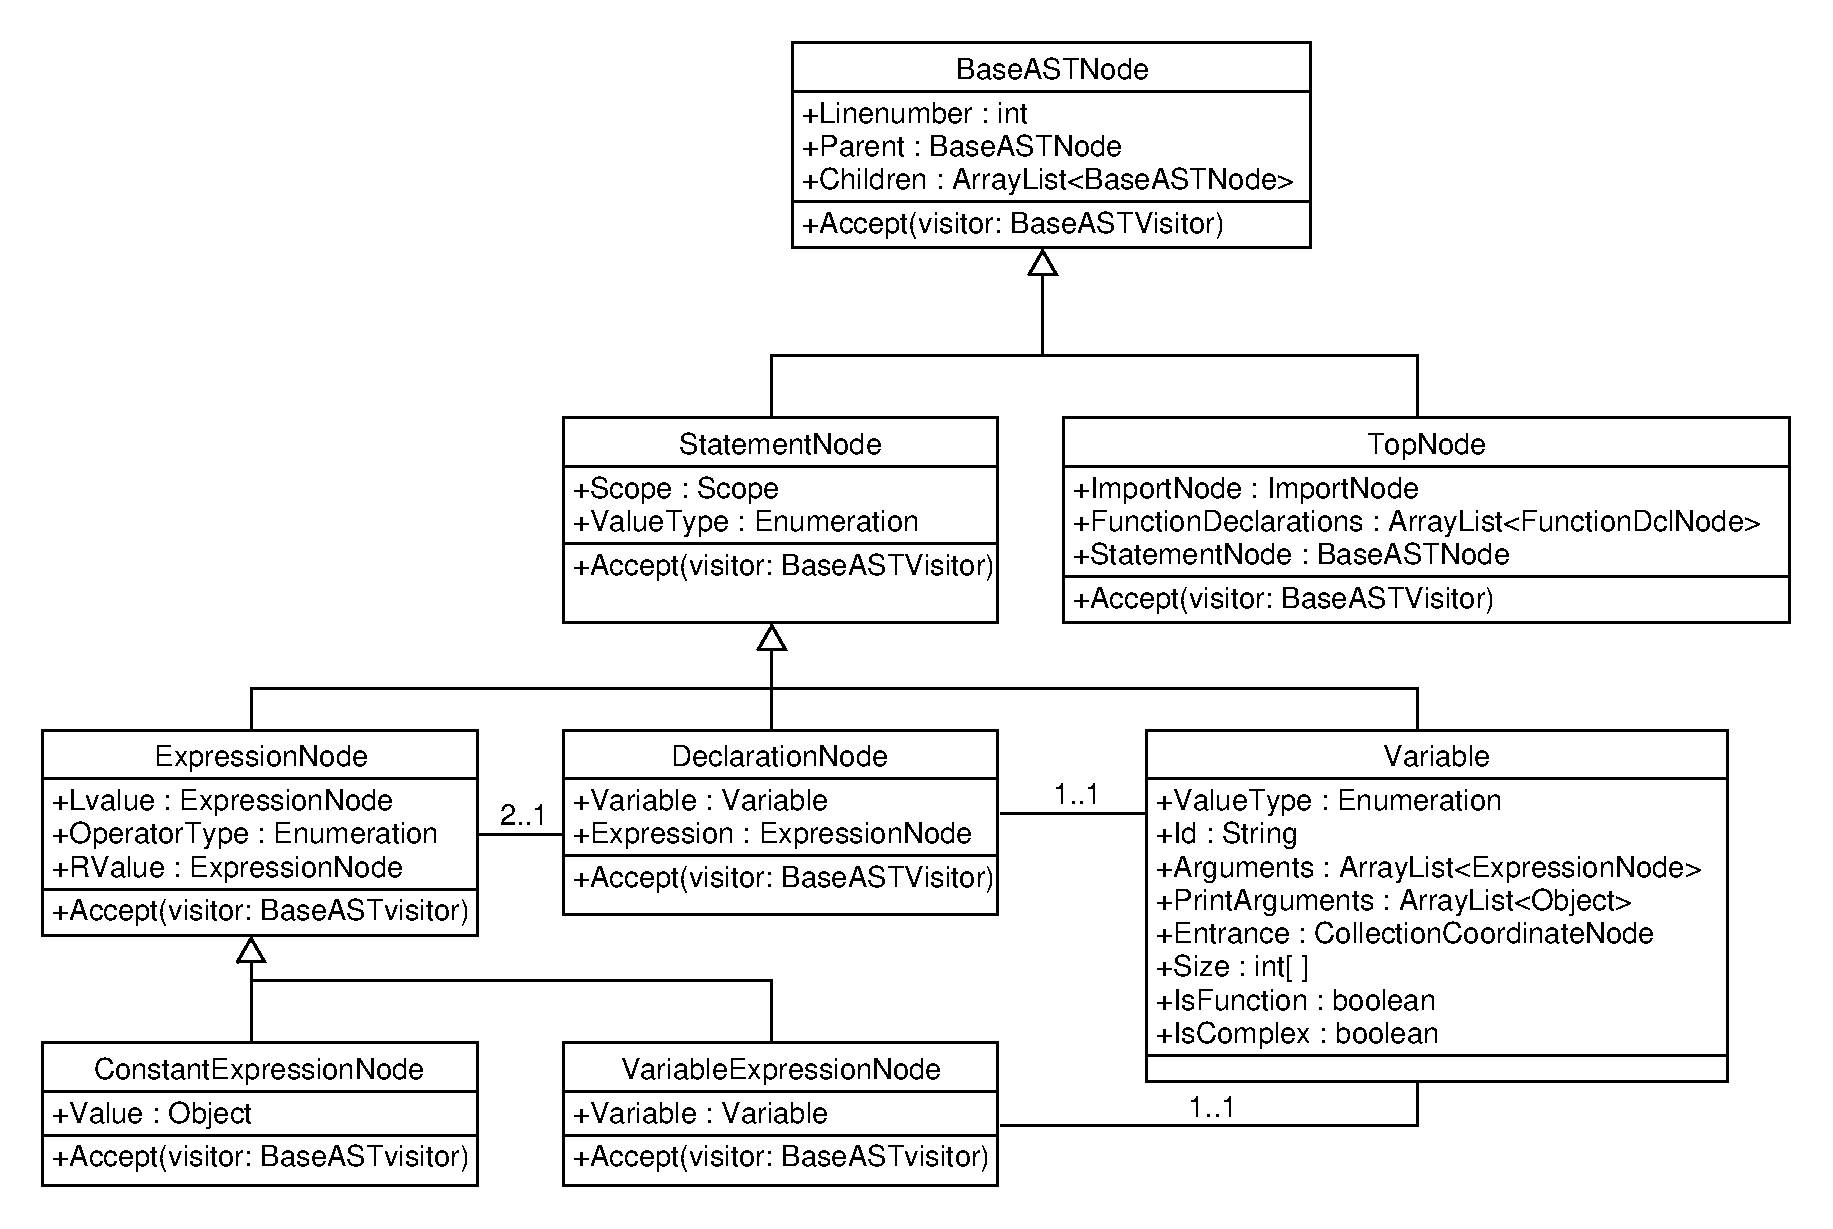
\includegraphics[width=1\textwidth]{figures/ClassDiagrams/ASTDeclarationNodeMoreInfo.pdf} % trim=4.85cm 15cm 0.85cm 1cm
\caption{A UML class diagram of the classes used for a DeclarationNode on the \acrshort{ast}.}\label{image:ASTDecl}
\vspace{-15pt}
\end{figure}

The \texttt{Variable} class contains a lot of different information which is used depending on which class a given instance of \texttt{Variable} is connected to.
If \texttt{Variable} is connected to a \texttt{VariableExpressionNode}, the only fields used on the variable class is ValueType and Id, while the booleans IsFunction and IsComplex are set to false.
In the example \texttt{int a = 5;} the tree structure looks like the AST on \myref{image:AST}.
When the right hand side of an assignment or declaration is a function, an example being \texttt{int a = foo(5);} the fields used on \texttt{Variable} differs from the previous example and instead becomes Id, ValueType, arguments, and the boolean IsFunction is instead set to true.
The print argument field is used when a function call to \texttt{Print()} is made. 
Entrance, Size and IsComplex are used when dealing with the complex data types, vectors and matrices.
\texttt{TopNode} sets the structure of a \gls{gamble} program as described in \myref{subsec:Struc}.
The full class diagram can be seen in \myref{ASTNodes}.

The classes have made it more intuitive to perform a traversal of the tree based upon the names of the fields on the classes.
E.g. the \texttt{ForLoopNode} has fields named \texttt{Body}, \texttt{Initialize}, \texttt{Update}, and \texttt{Conditional}, these names have meaning instead of just being children on the node which will be helpful when implementing the rest of the compiler.

The syntax analysis phase returns the \acrshort{ast} so it can be used in the next phase. 
The design of the phase and the call from main can be seen on \myref{fig:syntaxphase}.\todo{call from main kunne thomas ikke lide. MP}
As can be seen the \texttt{ASTGeneratorVisitor} makes use of the classes shown in \myref{ASTNodes}.

\begin{figure}[ht]
  \centering
    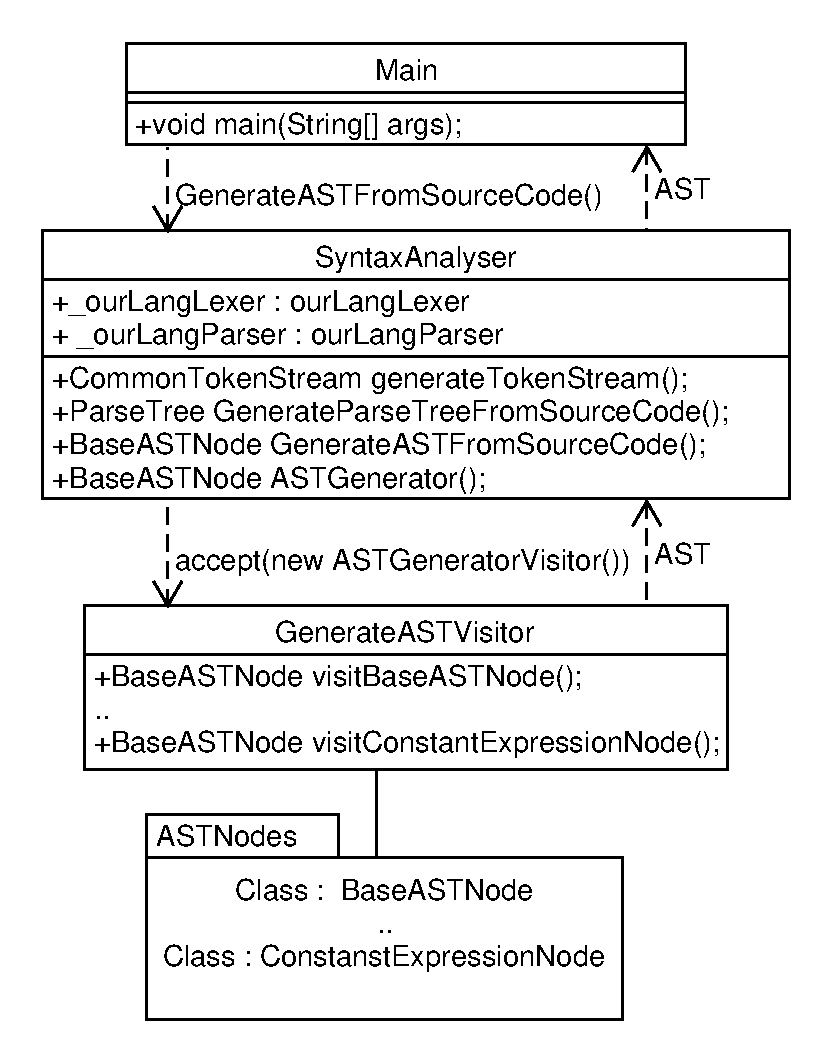
\includegraphics[width=0.48\textwidth]{figures/ClassDiagrams/SyntaxAnalyser.pdf}
  \caption{The function calls and returns in the Syntax Analysis phase.}
  \label{fig:syntaxphase}
\end{figure}